%\tcb{November 11}

Since the first implementation of the squeezing technique in a gravitational wave detector, which was realized at the GEO\,600 facility in 2010~\cite{GEOsqueezing}, numerous novel schemes regarding the long term application of squeezed light have been tested and implemented. These include, for example, the generation of the squeezing phase control signals \cite{Dooley2015} and the automatic alignment of the squeezed light field with respect to the interferometer \cite{Schreiber2016}, as well as ultra-low noise detection electronics \cite{Grote2016}. This led to a constant improvement of measured non-classical sensitivity enhancement \cite {Grote2013,Dooley2016}. In 2019 an effective squeezing level of 6\,dB could be measured at GEO\,600, which was a worlds first in a suspended gravitational wave interferometer. 
The Advanced Virgo and Advanced LIGO detectors have undergone upgrades that also contained the implementation of squeezed light leading to an average detected squeezing level between 2--3\,dB during the third joint LIGO-Virgo observations run O3. 
%
The great potential of including the squeezed light technique in the baseline design of ET becomes evident in Fig.\ref{QNSQZvsPNandloss}. In order to reach the goal of an effective 10\,dB quantum noise reduction, the overall optical loss for the squeezed field needs to be smaller than 10\,\% while the phase noise does not exceed 10\,mrad in total. 
%
\begin{wrapfigure}{r}{0.5\textwidth}
	\centering
		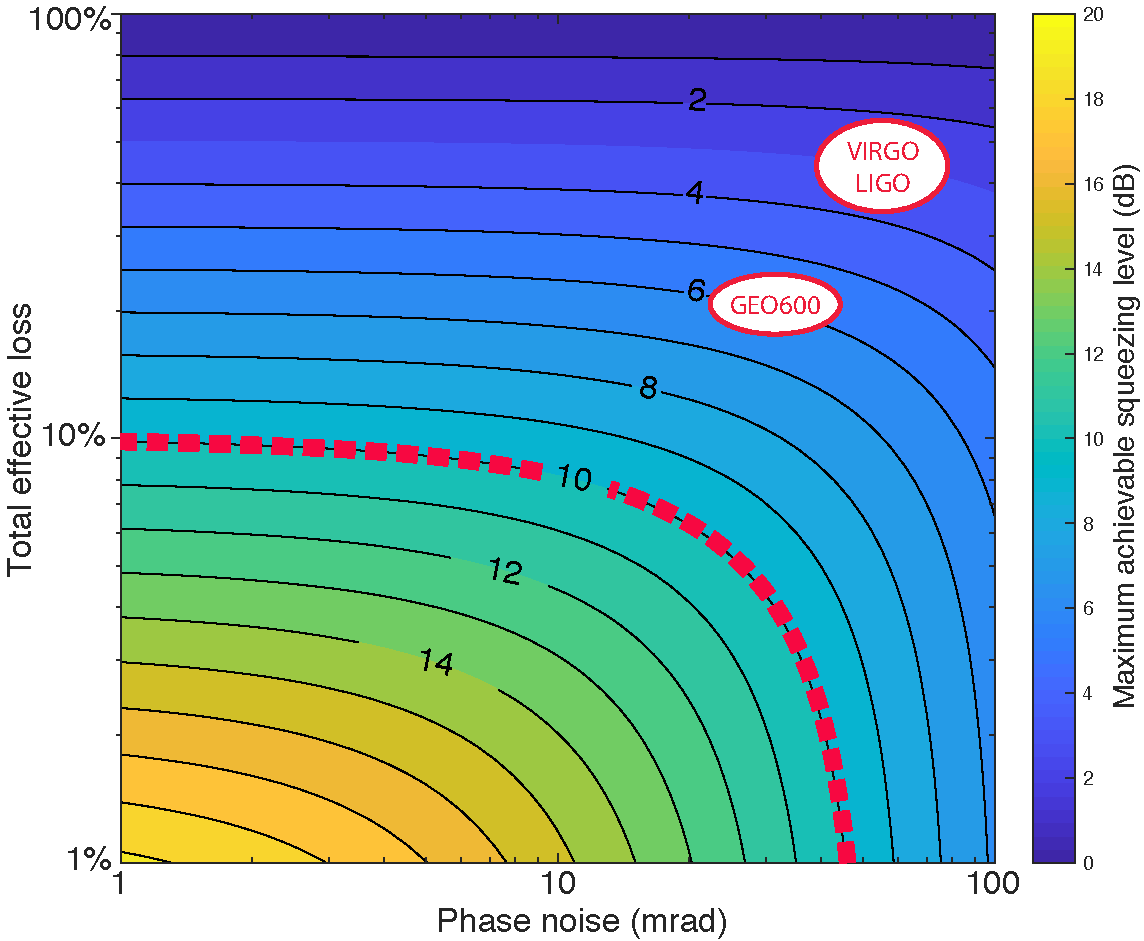
\includegraphics[width=0.5\textwidth]{./Detector/DetFigures/QNSQZvsPNandLoss.pdf}
	\caption{Maximum effective squeezing level as function of phase noise and optical loss. In order to reach the goal of 10\,dB detected squeezing, the optical loss needs to be smaller than 10\,\% while the phase noise must not exceed 10\,mrad.}
	\label{QNSQZvsPNandloss}
\end{wrapfigure}
%
The current generation of detectors achieve their exquisite sensitivity due to their kilometre-scale arm lengths, the enormous light powers circulating in the enhancement resonators (arm, power- and signal-recycling cavities), and sophisticated pendulum suspensions that isolate the test mass mirrors from the environment. When these techniques were developed, squeezing was not envisioned to become an integral part of such a system. However, the sensitivity improvements achieved already today via the injection of squeezed light (as an upgrade / add-on) are significant. For GEO\,600 an effective squeezing level of 6\,dB has been detected in the shot noise limited frequency band. As shown in Fig.\ref{QNSQZvsPNandloss} this corresponds to 25\,\% optical loss with a phase jitter of the squeezing ellipse of around 30\,mrad. A further reduction of optical loss and phase noise, the improvement in mode matching of the squeezed field to the interferometer signal field and mitigation of polarization mismatches will improve the effective quantum noise reduction even more in the future.
%
During the O3 science run both Advanced LIGO detectors and the Advanced VIRGO detector have not only been limited by quantum shot noise at high frequencies but have also operated close to being limited by quantum radiation pressure noise at lower detection frequencies. As a consequence, the injected squeezing level can not be increased to improve the high frequency sensitivity without degrading the detector sensitivity at lower frequencies and vice versa. 
%
It was revealed by Unruh~\cite{Unruh1982} and others~\cite{Yuen1983, Pace1993} that squeezed field injection with frequency dependent squeezing angle allows an overall quantum noise reduction including the radiation pressure noise thereby beating the standard quantum limit (SQL). The effect of a simultaneous suppression of quantum noise by means of a frequency dependent orientation of the squeezing ellipse (i.e. the correct squeezing phase for all detection frequencies) is illustrated in Fig.~\ref{UnruhFDS}.
%
%
\begin{wrapfigure}{l}{0.5\textwidth}
	\centering
		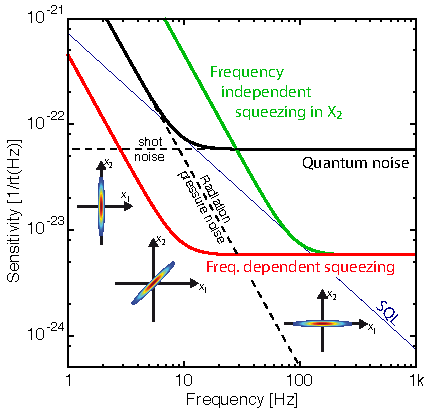
\includegraphics[width=0.5\textwidth]{./Detector/DetFigures/UnruhFDS.pdf}
	\caption[Illustration of frequency dependent and independent squeezed light injection]{Illustration of frequency dependent and independent squeezed light injection.}
	\label{UnruhFDS}
\end{wrapfigure}
%
For Advanced Virgo and Advanced LIGO, this can be realized with a detuned filter cavity and the corresponding technology is currently under development and planned to be implemented before the science run O4.  
%
The ET detectors will be quantum noise limited over the entire detection band and therefore suitable filter cavities have to be implemented. For the squeezed light injection into an optical spring interferometer, an additional rotation of the squeezing ellipse is caused first by the phase-space rotation of a detuned cavity and second due to the optical spring resonance. In this case at least two filter cavities are necessary to achieve a broadband reduction of quantum noise with squeezed states of light. This is what we propose for the low-frequency ET-LF interferometer (cf. Sec.~\ref{sec:xylophone}). For the high-frequency ET-HF interferometer one filter cavity is enough (cf. Sec.~\ref{sec:xylophone} and \cite{Hild2010b}).

The filter cavity assisted rotation of the squeezing ellipse has been experimentally demonstrated
in table top experiments both at MHz ~\cite{Chelkowski2005} and kHz \cite{Oelker2016} frequencies. However,
(0.1--1)\,km class filter cavities are required for long arm interferometers. For this reason a first prototype based on a 300\,m cavity is currently under test at the National Observatory of Japan (NAOJ) with the aim to obtain a rotation at approximately 70\,Hz ~\cite{Capocasa2019}.
Both collaborations LIGO \cite{McCuller2019} and VIRGO \cite{Degallaix2019} are presently working on the development of cavities of the same length scale. In general the optimal cavity length and parameters depend on the interferometer configuration. In this section we summarize the methods used for optimizing the filter cavities to be implemented in ET.

The use of filter cavities along the optical path of the squeezed light induces additional mechanisms and sources of squeezed light degradation which are in general frequency dependent. In optimizing the cavity design these detrimental effects must be taken into account: 

\textit{Filter cavity round trip loss --} The most relevant squeezing degradation mechanism comes from the filter cavity round trip losses which induce two effects: first optical loss mixes non-squeezed contributions into the squeezed vacuum state which leads to a degradation of the resulting squeezing level. Second the presence of filter cavity losses combined with the frequency dependent reflectivity mixes the two quadratures thereby corrupting squeezing with anti-squeezing. This effect cannot be compensated by a rotation of the state and therefore definitively deteriorates the actual quantum noise reduction ~\citep{Kwee2014}. To limit the impact of these effects the relevant parameter to be minimized is the cavity round trip loss per unit length $l^2_{rt-fc}/L_{fc}$ \cite{Khalili2010}. Therefore in order to keep the filter cavities length to an acceptable value the round trip losses must be minimized. 
% 
\begin{figure}%[ht]
\centering
\includegraphics[width=68mm]{./Detector/DetFigures/Mirror_Map.png} 
\includegraphics[width=75mm]{./Detector/DetFigures/FC_Stray.png}
\caption{{\it Left}: Virgo end  mirror surface map. The elements of the map represent the surface height deviation from a perfectly spherical mirror in meters ({\it provided by J. Degallaix/LMA}). {\it Right}: Expected cavity round trip losses as a function of the radius of curvature (RoC) of the mirrors for a 500\,m long linear cavity, equipped with Virgo-like mirrors (left plot) 200 mm in diameter ({\it credits M. Eisenmann)}. The background value derives from the light scattered outside the cavity, while the peaks originate from scattered light that couple to the high order modes of the cavity. The calculation is based on the method used in Ref.\citep{Capocasa2016} }
\label{fig:FC_rt_strain}
\end{figure}
%
Round trip cavity losses ($l^2_{fc-rt}$) are generally dominated by light scattering on the cavity  mirror surfaces. For this reason among the possible filter cavities configurations the {\it linear} cavity, which minimizes the number of mirrors, is preferable \cite{Evans2013}.  Recent measurements show that 50--90\,ppm can be achieved in 300\,m long linear cavities \citep{Capocasa2018}, a similar result (<60 ppm) has been obtained  for the VIRGO long arms.  Moreover, in the near future a further decrease in the scattering losses is foreseen. Indeed a numerical calculation shows that  with the latest  mirror quality and by optimizing their  diameter and radius of curvarure, scattering losses for a 500\,m long cavity can be constrained to 5--10\,ppm ( Fig.\ref{fig:FC_rt_strain} {\it right}).
%
In this design report we assume for the cavity round trip losses the ultra-conservative value $l^2_{fc-rt}=75$ ppm. However, to illustrate also lower cavity losses Fig.\ref{fig:FCoptimization} shows the quantum noise reduction, which can be expected for filter cavities with round trip losses in the range 40--75\,ppm. 
%
\begin{figure}%[htbp] \centering 
\includegraphics[width=77mm]{./Detector/DetFigures/ET_FC.png}
\includegraphics[width=77mm]{./Detector/DetFigures/FClength.png}
\caption{ {\it Left:} Ratio between the quantum noise with and without squeezed light injection for a 500\,m long cavity. Several (colored curves) degradation mechanisms contribute to the total squeezing degradation budged (black curve). The dominant contribution at low frequencies derives from the round trip losses of the cavity (yellow curve). The values assumed for the cavity round trip losses range from 40\,ppm to\,75 ppm. {\it Right:} Total degradation budget for different cavity lengths ({\it credits E. Capocasa}).} 
\label{fig:FCoptimization}
\end{figure} 
%

\textit{Mode mismatch --} A non-perfect spatial overlap (mode mismatch) between the squeezed beam and the eigenmode of the filter cavity
 is a source of optical loss, which is independent from the filter cavity length. 
 The target mode matching value of ET is $\sim 98\%$, analog to the LIGO and VIRGO quantum noise reduction projects.

\textit{Phase noise --} The achievable sensitivity improvement by injecting squeezed light is deteriorated due to phase noise between the interferometer carrier and the squeezed field. The suspended filter cavity can produce phase noise due to residual changes of the cavity length $\delta L_{fc}$ which generate fluctuations in the detuning frequency $\Delta \omega_{fc}$:
%
%Except for intra-cavity fluctuations phase noise is in general frequency independent.  
%A typical intra-cavity fluctuation is generated by the residual displacement noise $\delta L_{fc}$ of the cavity length which generates fluctuations in the detuning frequency $\delta \Delta \omega_{fc}$.
%
  \begin{equation}
    \delta \Delta \omega_{fc}=\omega_0 \frac{\delta L_{fc}}{L_{fc}} \ .
  \end{equation}
For this work we assume $\delta L_{fc}=0.1$\,pm. which is  within the reach of current technologies.

Figure \ref{fig:FCoptimization}-{\it left} shows the level of quantum noise reduction as a function of frequency for the ET-HF configuration. %(table...). 
The optimal cavity bandwidth $\gamma_{\rm fc}$ (half-width at half-maximum) and detuning $\Delta \omega_{\rm fc}$ are calculated analytically according to Ref. \cite{Kwee2014}. 
Figure \ref{fig:FCoptimization}-{\it right} shows that the quantum noise reduction increases by extending the cavity length. However, this effect is less and less pronounced as one approaches frequencies beyond the cavity bandwidth, where the sources for squeezing degradation are filter cavity length-independent. Moreover, at low frequencies additional technical noise sources contribute significantly to the overall detector sensitivity and thus a strong quantum noise suppression is not observable and hence not required. A short cavity design is therefore well suited for an efficient high frequency quantum noise reduction, with a reduced suppression at low frequencies. This strategy also minimizes the costs and complexity and is therefore applied to the ET-filter-cavity designs.

A similar optimization was also used for the two cavities of the detuned configuration as planned for ET-LF. However, to our knowledge in this case no analytical expression for the optimal cavity bandwidth and detuning is available in presence of losses. Therefore the optimization was done numerically. 
This optimization process led to the choice of a length of 500 meters for the ET-HF filter cavity and 1000 meters for the two ET-LF cavities.